\chapter{CLAW-FREE GRAPHS}\label{ClawFreeChapter}
\begin{center}
\emph{Some of the material in this chapter appeared in \cite{cranstonrabernclaw} and is joint work with Dan Cranston.}
\end{center}

In \cite{dhurandhar1982improvement}, Dhurandhar proved the Borodin-Kostochka
Conjecture for a superset of line graphs of \emph{simple} graphs defined by excluding the claw, $K_5 - e$ and another graph $D$ as induced subgraphs.  
Kierstead and Schmerl \cite{kierstead1986chromatic} improved this by removing
the need to exclude $D$.  The aim of this chapter is to remove the need to exclude $K_5 - e$; that is, to prove the Borodin-Kostochka
Conjecture for claw-free graphs.

\begin{repthm}{BKClawFree}
Every claw-free graph satisfying $\chi \geq \Delta \geq 9$ contains a
$K_\Delta$.
\end{repthm}

This also generalizes the result of Beutelspacher and Hering \cite{beutelspacher1984minimal} that the
Borodin-Kostochka conjecture holds for graphs with independence number at most
two.  The value of $9$ in Theorem \ref{BKClawFree} is best possible since the
counterexample for $\Delta = 8$ in Figure \ref{fig:SmallCE} is claw-free.
Theorem \ref{BKClawFree} is also optimal in the following sense.  We can
reformulate the statement as: every claw-free graph with $\Delta \geq 9$
satisfies $\chi \leq \max\{\omega, \Delta - 1\}$.  Consider a similar statement
with $\Delta - 1$ replaced by $f(\Delta)$ for some $\func{f}{\IN}{\IN}$ and $9$
replaced by $\Delta_0$. We show that $f(x) \geq x - 1$ for $x \geq \Delta_0$. 
Consider $G_t \DefinedAs \join{K_t}{C_5}$.  We have $\chi(G_t) = t + 3$, $\omega(G_t) = t + 2$
and $\Delta(G_t) = t + 4$ and $G_t$ is claw-free.  Hence for $t \geq \Delta_0
- 4$ we have $t + 3 \leq \max\set{t + 2, f(t + 4)} \leq f(t + 4)$ giving $f(x)
\geq x - 1$ for $x \geq \Delta_0$.

As shown in \cite{rabern2011strengthening} (also Section \ref{LineGraphSection}) the situation is very different for
line graphs of multigraphs which satisfy $\chi \leq \max\{\omega,
\frac{7\Delta + 10}{8}\}$.  There it was conjectured that $f(x) \DefinedAs
\frac{5x + 8}{6}$ works for line graphs of multigraphs; this would be best
possible.  The example of $\join{K_t}{C_5}$ is claw-free, but it isn't
quasi-line.

\begin{question}
What is the situation for quasi-line graphs?  That is, what is the optimal
$f$ such that every quasi-line graph with large enough maximum degree satisfies
$\chi \leq \max\{\omega, f(\Delta)\}$.
\end{question}

\section{Line graphs}\label{LineGraphSection}
\begin{center}
\emph{The material in this section appeared in \cite{rabern2011strengthening}.}
\end{center}

In this section we prove the Bornodin-Kostochka Conjecture for line graphs of \emph{multigraphs}.  Moreoever, we prove a strengthening of Brooks' theorem for line graphs of multigraphs and conjecture the best possible such bound.

\begin{lem}\label{muBoundLemma}
Fix $k \geq 0$. Let $H$ be a multigraph and put $G = L(H)$.  Suppose $\chi(G) = \Delta(G) + 1 - k$. If $xy \in E(H)$ is critical and $\mu(xy) \geq 2k + 2$, then $xy$ is contained in a $\chi(G)$-clique in $G$.
\end{lem}
\begin{proof}
Let $xy \in E(H)$ be a critical edge with $\mu(xy) \geq 2k + 2$.  Let $A$ be the set of all edges incident with both $x$ and $y$.  Let $B$ be the set of edges incident with either $x$ or $y$ but not both.  Then, in $G$, $A$ is a clique joined to $B$ and $B$ is the complement of a bipartite graph.  Put $F = G[A \cup B]$.  Since $xy$ is critical, we have a $\chi(G) - 1$ coloring of $G - F$.  Viewed as a partial $\chi(G) - 1$ coloring of $G$ this leaves a list assignment $L$ on $F$ with 
$|L(v)| = \chi(G) - 1 - (d_G(v) - d_F(v)) = d_F(v) - k + \Delta(G) - d_G(v)$ for each $v \in V(F)$.  Put $j = k + d_G(xy) - \Delta(G)$.

Let $M$ be a maximum matching in the complement of $B$.  First suppose $|M| \leq j$.  Then, since $B$ is perfect, $\omega(B) = \chi(B)$ and we have

\begin{align*}
\omega(F) &= \omega(A) + \omega(B) = |A| + \chi(B) \\
&\geq |A| + |B| - j = d_G(xy) + 1 - j \\
&= \Delta(G) + 1 - k = \chi(G).
\end{align*}

\noindent Thus $xy$ is contained in a $\chi(G)$-clique in $G$.

Hence we may assume that $|M| \geq j + 1$.  Let $\{\{x_1, y_1\}, \ldots, \{x_{j+1}, y_{j+1}\}\}$ be a matching in the complement of $B$.  Then, for each $1 \leq i \leq j + 1$ we have

\begin{align*}
|L(x_i)| + |L(y_i)| &\geq d_F(x_i) + d_F(y_i) - 2k \\
&\geq |B| - 2 + 2|A| - 2k \\
&= d_G(xy) + |A| - 2k - 1 \\
&\geq d_G(xy) + 1.
\end{align*}

Here the second inequality follows since $\alpha(B) \leq 2$ and the last since $|A| = \mu(xy) \geq 2k + 2$.  Since the lists together contain at most $\chi(G) - 1 = \Delta(G) - k$ colors we see that for each $i$,

\begin{align*}
\left|L(x_i) \cap L(y_i)\right| &\geq |L(x_i)| + |L(y_i)| - (\Delta(G) - k) \\
&\geq d_G(xy) + 1 - \Delta(G) + k \\
&=j + 1.
\end{align*}

Thus we may color the vertices in the pairs $\{x_1, y_1\}, \ldots, \{x_{j+1}, y_{j+1}\}$ from $L$ using one color for each pair.  Since $|A| \geq k + 1$ we can extend this to a coloring of $B$ from $L$ by coloring greedily.  But each vertex in $A$ has $j+1$ colors used twice on its neighborhood, thus each vertex in $A$ is left with a list of size at least $d_A(v) - k + \Delta(G) - d_G(v) + j + 1 = d_A(v) + 1$.  Hence we can complete the $(\chi(G) - 1)$-coloring to all of $F$ by coloring greedily.  This contradiction completes the proof.
\end{proof}

\begin{thm}\label{CriticalMuBound}
If $G$ is the line graph of a multigraph $H$ and $G$ is vertex critical, then
\[\chi(G) \leq \max\left\{\omega(G), \Delta(G) + 1 - \frac{\mu(H) - 1}{2}\right\}.\]
\end{thm}
\begin{proof}
Let $G$ be the line graph of a multigraph $H$ such that $G$ is vertex critical. Say $\chi(G) = \Delta(G) + 1 - k$.  Suppose $\chi(G) > \omega(G)$.  Since $G$ is vertex critical, every edge in $H$ is critical.  Hence, by Lemma \ref{muBoundLemma}, $\mu(H) \leq 2k+1$.  That is, $\mu(H) \leq 2(\Delta(G) + 1 - \chi(G)) + 1$.  The theorem follows.
\end{proof}

This upper bound is tight.  To see this, let $H_t = t \cdot C_5$ (i.e. $C_5$ where each edge has multiplicity $t$) and put $G_t = L(H_t)$.  As Catlin \cite{catlin1979hajos} showed, for odd $t$ we have $\chi(G_t) = \frac{5t + 1}{2}$, $\Delta(G_t) = 3t - 1$, and $\omega(G_t) = 2t$.  Since $\mu(H_t) = t$, the upper bound is achieved.

\noindent We need the following lemma which is a consequence of the fan equation (see \cite{anderson1977edge, cariolaro2006fans, StiebitzVizingGoldberg, GoldbergJGT}).
\begin{lem}\label{FanEquation}
Let $G$ be the line graph of a multigraph $H$.  Suppose $G$ is vertex critical with $\chi(G) > \Delta(H)$. Then, for any $x \in V(H)$ there exist $z_1, z_2 \in N_H(x)$ such that $z_1 \neq z_2$ and 
\begin{itemize}
\item $\chi(G) \leq d_H(z_1) + \mu(xz_1)$,
\item $2\chi(G) \leq d_H(z_1) + \mu(xz_1) + d_H(z_2) + \mu(xz_2)$.
\end{itemize}
\end{lem}

\begin{lem}\label{Goldberg}
Let $G$ be the line graph of a multigraph $H$.  If $G$ is vertex critical with $\chi(G) > \Delta(H)$, then
\[\chi(G) \leq \frac{3\mu(H) + \Delta(G) + 1}{2}.\]
\end{lem}
\begin{proof}
Let $x \in V(H)$ with $d_H(x) = \Delta(H)$.  By Lemma \ref{FanEquation} we have $z \in N_H(x)$ such that $\chi(G) \leq d_H(z) + \mu(xz)$.  Hence
\[\Delta(G) + 1 \geq d_H(x) + d_H(z) - \mu(xz) \geq d_H(x) + \chi(G) - 2\mu(xz).\]

\noindent Which gives

\[\chi(G) \leq \Delta(G) + 1 - \Delta(H) + 2\mu(H).\]

\noindent Adding Vizing's inequality $\chi(G) \leq \Delta(H) + \mu(H)$ gives the desired result.
\end{proof}

\noindent Combining this with Theorem \ref{CriticalMuBound} we get the following upper bound.

\begin{thm}\label{TheoremL}
If $G$ is the line graph of a multigraph, then
\[\chi(G) \leq \max\left\{\omega(G), \frac{7\Delta(G) + 10}{8}\right\}.\]
\end{thm}
\begin{proof}
Suppose not and choose a counterexample $G$ with the minimum number of vertices.  Say $G = L(H)$. Plainly, $G$ is vertex critical.  Suppose $\chi(G) > \omega(G)$. By Theorem \ref{CriticalMuBound} we have

\[\chi(G) \leq \Delta(G) + 1 - \frac{\mu(H) - 1}{2}.\]

\noindent By Lemma \ref{Goldberg} we have

\[\chi(G) \leq \frac{3\mu(H) + \Delta(G) + 1}{2}.\]

\noindent Adding three times the first inequality to the second gives

\[4\chi(G) \leq \frac72(\Delta(G) + 1) + \frac32.\]

\noindent The theorem follows.
\end{proof}

\begin{cor}
If $G$ is the line graph of a multigraph with $\chi(G) \geq \Delta(G) \geq 11$, then $G$ contains a $K_{\Delta(G)}$.
\end{cor}

With a little more care we can get the $11$ down to $9$.  Using Lemma \ref{HereditaryReduction}, we can inductively reduce to the $\Delta = 9$ case.

\begin{thm}\label{BKLineGraph}
If $G$ is the line graph of a multigraph with $\chi(G) \geq \Delta(G) \geq 9$, then  $G$ contains a $K_{\Delta(G)}$.
\end{thm} 
\begin{proof}

Suppose the theorem is false and choose a counterexample $G$ minimizing $\Delta(G)$.  Then $G$ is vertex critical.  By Lemma \ref{HereditaryReduction}, $\Delta(G) = 9$.

Let $H$ be such that $G = L(H)$.  Then by Lemma \ref{muBoundLemma} and Lemma \ref{Goldberg} we know that $\mu(H) = 3$. Let $x \in V(H)$ with $d_H(x) = \Delta(H)$.  Then we have $z_1, z_2 \in N_H(x)$ as in Lemma \ref{FanEquation}.  This gives
\begin{eqnarray}
9 &\leq& d_H(z_1) + \mu(xz_1), \\
18 &\leq& d_H(z_1) + \mu(xz_1) + d_H(z_2) + \mu(xz_2).
\end{eqnarray}

\noindent In addition, we have for $i = 1,2$, 

\[9 \geq d_H(x) + d_H(z_i) - \mu(xz_i) - 1 = \Delta(H) + d_H(z_i) - \mu(xz_i) - 1.\]

\noindent Thus,

\begin{eqnarray}
\Delta(H) &\leq& 2\mu(xz_1) + 1 \leq 7, \\
\Delta(H) &\leq& \mu(xz_1) + \mu(xz_2) + 1.
\end{eqnarray}

Now, let $ab \in E(H)$ with $\mu(ab) = 3$.  Then, since $G$ is vertex critical, we have $8 = \Delta(G) - 1 \leq d_H(a) + d_H(b) - \mu(ab) - 1 \leq 2\Delta(H) - 4$.  Thus $\Delta(H) \geq 6$.  Hence we have $6 \leq \Delta(H) \leq 7$.  Thus, by $(3)$, we must have $\mu(xz_1) = 3$.

First, suppose $\Delta(H) = 7$.  Then, by $(4)$ we have $\mu(xz_2) = 3$.  Let $y$ be the other neighbor of $x$.  Then $\mu(xy) = 1$ and thus $d_H(x) + d_H(y) - 2 \leq 9$.  That gives $d_H(y) \leq 4$.  Then we have vertices $w_1, w_2 \in N_H(y)$ guaranteed by Lemma \ref{FanEquation}. Note that $x \not \in \{w_1, w_2\}$.  Now $4 \geq d_H(y) \geq 1 + \mu(yw_1) + \mu(yw_2)$.  Thus $\mu(yw_1) + \mu(yw_2) \leq 3$.  This gives $d_H(w_1) + d_H(w_2) \geq 2\Delta(G) - 3 = 15$ contradicting $\Delta(H) \leq 7$.

Thus we must have $\Delta(H) = 6$.  By $(1)$ we have $d_H(z_1) = 6$.  Then, applying $(2)$ gives $\mu(xz_2) = 3$ and $d_H(z_2) = 6$.  Since $x$ was an arbitrary vertex of maximum degree and $H$ is connected we conclude that $G = L(3\cdot C_n)$ for some $n \geq 4$.  But no such graph is $9$-chromatic by Brooks' theorem.
\end{proof}

The graphs $G_t = L(t \cdot C_5)$ discussed above show that the following upper bound would be tight.  Creating a counterexample would require some new construction technique that might lead to more counterexamples to Borodin-Kostochka for $\Delta=8$.

\begin{conjecture}\label{BestPossibleWithJustDelta}
If $G$ is the line graph of a multigraph, then
\[\chi(G) \leq \max\left\{\omega(G),\frac{5\Delta(G) + 8}{6}\right\}.\]
\end{conjecture}

\section{Circular interval graphs}
A \emph{representation} of a graph $G$ in a graph $H$ consists of: 

\begin{itemize}
  \item an injection $\funcinj{f}{V(G)}{V(H)}$;
  \item for each $xy \in E(G)$, a choice of path $p_{xy} \subseteq H$ from
  $f(x)$ to $f(y)$ such that $f^{-1}(V(p_{xy}))$ is a clique in $G$.
\end{itemize}

A graph is a \emph{circular interval graph} if it has a representation in a
cycle. We note that this class coincides with the class of proper circular arc
graphs.  A graph is a \emph{linear interval graph} if it has a representation in
a path.

\begin{lem}\label{CircularIntervalLemma}
Every circular interval graph satisfying $\chi_l \ge \Delta \ge 9$ contains a
$K_\Delta$.
\end{lem}
\begin{proof}
Suppose the contrary and choose a counterexample $G$ minimizing $\card{G}$.  Put
$\Delta \DefinedAs \Delta(G)$. Then $\chi_l(G)=\Delta$, $\omega(G)\le \Delta-1$,
$\delta(G)\ge \Delta-1$ and $\chi_l(G-v)\le \Delta-1$ for all $v\in V(G)$. 
%We call $\Delta$-vertices \textit{high} and $(\Delta-1)$-vertices \textit{low}.
Since $G$ is a circular interval graph, by definition $G$ has a representation
in a cycle $v_1v_2\ldots v_n$.  Let $K$ be a maximum clique in $G$.  By symmetry we may assume that
$V(K)=\{v_1,v_2,\ldots,v_t\}$ for some $t\le \Delta-1$; further, if possible we
label the vertices so that $v_{t-3}\adj v_{t+1}$ and the edge goes through
$v_{t-2},v_{t-1},v_t$.

\textbf{Claim 1.} \textit{$v_1\nonadj v_{t+1}$ and $v_2\nonadj v_{t+2}$ and
$v_1\nonadj v_{t+2}$}. 
Suppose the contrary.
Clearly we can't have $v_1\adj v_{t+1}$ and have the edge go through
$v_2,v_3,\ldots, v_t$ (since then we get a clique of size $t+1$).
Similarly, we can't have $v_2\adj v_{t+2}$ and have the edge go through
$v_3,v_4,\ldots,v_{t+1}$.  So assume the edge $v_1v_{t+2}$ exists and 
goes around the other way.
If $v_1\adj v_{t+1}$, then let $G'=G\setminus \{v_1\}$ and if $v_1\nonadj
v_{t+1}$, then let $G'=G\setminus \{v_1,v_{t+1}\}$.  Now let
$V_1=\{v_2,v_3,\ldots,v_t\}$ and $V_2=V(G')\setminus V_1$.  Let $K'=G[V_1]$ and
$L'=G[V_2]$; note that $K'$ and $L'$ are each cliques of size at most
$\Delta-2$.  Now for each $S\subseteq V_2$,
we have $|N_{\overline{G}}(S)\cap V_1|\ge |S|$
%there exists $T\subseteq V_1$ with $|T|=|S|$ such that for each $v\in T$ there
%exists $u\in S$ such that $u\nonadj v$ 
(otherwise we get a clique of size $t$ in $G'$ and a clique of size $t+1$ in $G$).  Now by Hall's Theorem, we have a matching in $\overline{G}$ between $V_1$
and $V_2$ that saturates $V_2$.  This implies that $G'\subseteq E_2^{\Delta-2}$,
which in turn gives $G\subseteq E_2^{\Delta-1}$.  By Lemma~\ref{E2n}, $G$ is
$(\Delta-1)$-choosable, which is a contradiction.

\textbf{Claim 2.} \textit{$v_{t-3}\adj v_{t+1}$ and the edge passes through
$v_{t-2},v_{t-1},v_t$.}
Suppose the contrary.
If $t\ge 7$, then since $t\le \Delta-1$, $v_4$ has some
neighbor outside of $K$; by (reflectional) symmetry we could have labeled the
vertices so that $v_{t-3}\adj v_{t+1}$.
So we must have $t\le 6$.
Each vertex $v$ that is high has either at least $\ceil{\Delta/2}$ clockwise
neighbors or at least $\ceil{\Delta/2}$ counterclockwise neighbors.  This gives a clique
of size $1+\ceil{\Delta/2}\ge 6$.  If $v_3$ is high, then either $v_3$ has at
least 4 clockwise neighbors, so $v_3\adj v_7$, or else $v_3$ has at least 6
counterclockwise neighbors, so $|K|\ge 7$.  Thus, we may assume that $v_3$ is
low; by symmetry (and our choice of labeling prior to Claim~1) $v_4$ is also
low.  Now since $v_4$ has only 3 counterclockwise neighbors, we get $v_4\adj
v_7$ (in fact, we get $v_4\adj v_9$).  Thus, $\{v_3,v_4,v_5,v_6,v_7\}$ induces
$K_3*E_2$ with a low degree vertex in both the $K_3$ and the $E_2$, which 
contradicts Lemma~\ref{mixed3}.

\textbf{Claim 3.} \textit{$v_{t-2} \nonadj v_{t+2}$}.  Suppose the contrary.  By
Claim~1 the edge goes through $v_{t-1},v_t,v_{t+1}$.  If $v_{t-3}\adj v_{t+2}$,
then $\{v_1,v_2,v_{t-3},v_{t-2},v_{t-1},v_t,v_{t+1},v_{t+2}\}$ induces $K_4*B$,
where $B$ is not almost complete; this contradicts
Lemma~\ref{ConnectedAtLeast4Poss}.  If $v_{t-3}\nonadj v_{t+2}$, then we get a
$K_3*P_4$ induced by $\{v_1, v_{t-3}, v_{t-2}, v_{t-1}, v_t, v_{t+1},
v_{t+2}\}$, which contradicts Lemma~\ref{K3P4}. 

\textbf{Claim 4.} \textit{$v_{t-1}\nonadj v_{t+2}$}.  
If not, then $\{v_1,v_{t-3},v_{t-2},v_{t-1},v_t, v_{t+1}, v_{t+2}\}$ induces
$K_2*\mbox{antichair}$ (with $v_{t-1},v_t$ in the $K_2$), which contradicts
Lemma~\ref{K2Antichair}.

\textbf{Claim 5.} \textit{$G$ is $(\Delta-1)$-choosable.}  
Let $S=\{v_{t-3},v_{t-2},v_{t-1},v_t\}$.  If any vertex of $S$ is low, then
$S\cup\{v_1,v_{t+1}\}$ induces $K_4*E_2$ with a low vertex in the $K_4$, which
contradicts Lemma~\ref{mixed}.  So all of $S$ is high.  If
$v_t\nonadj v_{t+2}$, then $\{v_t,v_{t-1},\ldots, v_{t-\Delta+1}\}$ (subscripts
are modulo $n$) induces $K_{\Delta}$.  So $v_t\adj v_{t+2}$.  Since
$v_{t-1}\nonadj v_{t+2}$ and all of $S$ is high, we get $v_n\in (\cap_{v\in
(S\setminus\{v_t\})}N(v))\setminus N(v_t)$.  Now we must have $v_n\nonadj
v_{t+1}$ (for otherwise $G$ is $(\Delta-1)$-choosable, as in Claim~1).  So we
get $K_3*P_4$ induced by $\{v_{t+1},v_t,v_{t-1},v_{t-2},v_{t-3},v_1,v_n\}$,
which contradicts Lemma~\ref{K3Classification}.  
\end{proof}
\section{Quasi-line graphs}
A graph is \emph{quasi-line} if every vertex is bisimplicial (its neighborhood can be covered by two cliques).  
We apply a version of Chudnovsky and Seymour's structure theorem for quasi-line
graphs from King's thesis \cite{king2009claw}. The undefined terms
will be defined after the statement.

\begin{lem}\label{QuasilineStructure}
Every connected skeletal quasi-line graph is a circular interval graph or a composition of
linear interval strips.
\end{lem}

A \emph{homogeneous pair of cliques} $(A_1, A_2)$ in a graph $G$ is a pair of
disjoint nonempty cliques such that for each $i \in \irange{2}$, every vertex in
$G - (A_1 \cup A_2)$ is either joined to $A_i$ or misses all of $A_i$ and
$\card{A_1} + \card{A_2} \geq 3$. A homogeneous pair of cliques $(A_1, A_2)$ is $\emph{skeletal}$
if for any $e \in E(A, B)$ we have $\omega(G[A \cup B] - e) < \omega(G[A \cup
B])$.  A graph is $\emph{skeletal}$ if it contains no nonskeletal homogeneous
pair of cliques.

Generalizaing a lemma of Chudnovsky and Fradkin \cite{chudnovskyFradkin}, King
proved a lemma allowing us to handle nonskeletal homogeneous pairs
of cliques.

\begin{lem}[King \cite{king2009claw}]\label{NoHomogeneous} If $G$ is a
nonskeletal graph, then there is a proper subgraph $G'$ of $G$ such that:
\begin{enumerate}
  \item $G'$ is skeletal;
  \item $\chi(G') = \chi(G)$;
  \item If $G$ is claw-free, then so is $G'$;
  \item If $G$ is quasi-line, then so is $G'$.
\end{enumerate}
\end{lem}

It remains to define the generalization of line graphs introduced by Chudnovsky
and Seymour \cite{chudnovsky2005structure}; this is the notion of
\emph{compositions of strips} (for a more detailed introduction, see Chapter 5
of~\cite{king2009claw}). We use the modified definition from King and
Reed \cite{king2008bounding}. A \emph{strip} $(H, A_1, A_2)$ is a claw-free
graph $H$ containing two cliques $A_1$ and $A_2$ such that for each $i \in \irange{2}$ and $v \in A_i$, $N_H(v) - A_i$ is a clique.  
If $H$ is a linear interval graph, then $(H, A_1, A_2)$ is a $\emph{linear
interval strip}$.  Now let $H$ be a directed multigraph (possibly with loops)
and suppose for each edge $e$ of $H$ we have a strip $(H_e, X_e, Y_e)$.  For
each $v \in V(H)$ define

\[C_v \DefinedAs \parens{\bigcup \setbs{X_e}{\text{$e$ is directed out of $v$}}}
\cup \parens{\bigcup \setbs{Y_e}{\text{$e$ is directed into $v$}}}\]

The graph formed by taking the disjoint union of $\setbs{H_e}{e \in E(H)}$ and
making $C_v$ a clique for each $v \in V(H)$ is the composition of the strips
$(H_e, X_e, Y_e)$.  Any graph formed in such a manner is called a
\emph{composition of strips}.  It is easy to see that if for
each strip $(H_e, X_e, Y_e)$ in the composition we have $V(H_e) = X_e = Y_e$,
then the constructed graph is just the line graph of the multigraph formed by
replacing each $e \in E(H)$ with $\card{H_e}$ copies of $e$.

It will be convenient to have notation and terminology for a strip together with
how it attaches to the graph. An \emph{interval $2$-join} in a graph $G$ is an
induced subgraph $H$ such that:
\begin{enumerate}
\item $H$ is a (nonempty) linear interval graph,
\item The ends of $H$ are (not necessarily disjoint) cliques $A_1$, $A_2$,
\item $G-H$ contains cliques $B_1$, $B_2$ (not necessarily disjoint) such that $A_1$ is joined to $B_1$ and $A_2$ is joined to $B_2$,
\item there are no other edges between $H$ and $G-H$.
\end{enumerate}

Note that $A_1, A_2, B_1, B_2$ are uniquely determined by $H$, so we
are justified in calling both $H$ and the quintuple $(H, A_1, A_2, B_1, B_2)$
the interval $2$-join. An interval $2$-join $(H, A_1, A_2, B_1, B_2)$ is
\emph{trivial} if $V(H) = A_1 = A_2$ and \emph{canonical} if $A_1 \cap A_2 =
\emptyset$.  A canonical interval $2$-join $(H, A_1, A_2, B_1, B_2)$ with
leftmost vertex $v_1$ and rightmost vertex $v_t$ is \emph{reducible} if $H$ is
incomplete and $N_H(A_1)\setminus A_1 = N_H(v_1)\setminus A_1$ or
$N_H(A_2)\setminus A_2 = N_H(v_t)\setminus A_2$.  We call such a canonical
interval $2$-join reducible because we can \emph{reduce} it as follows.  Suppose
$H$ is incomplete and $N_H(A_1)\setminus A_1 = N_H(v_1)\setminus A_1$. Put $C
\DefinedAs N_H(v_1) \setminus A_1$ and then $A_1' \DefinedAs C \setminus A_2$ and $A_2' \DefinedAs A_2 \setminus C$.  
Since $H$ is not complete $v_t \in A_2'$ and hence $H' \DefinedAs G[A_1' \cup
A_2']$ is a nonempty linear interval graph that gives the reduced canonical
interval $2$-join $(H', A_1', A_2', A_1 \cup \parens{C \cap A_2}, B_2 \cup
\parens{C \cap A_2}$.

\begin{lem}\label{Irreducible2Join}
If $(H, A_1, A_2, B_1, B_2)$ is an irreducible canonical interval $2$-join in a
vertex critical graph $G$ with $\chi(G) = \Delta(G) \geq 9$, then $B_1 \cap B_2
= \emptyset$ and $\card{A_1}, \card{A_2} \leq 3$.  Moreover, if $G$ is skeletal,
then $H$ is complete.
\end{lem}
\begin{proof}
Let $(H, A_1, A_2, B_1, B_2)$ be an irreducible canonical interval $2$-join in a
vertex critical graph $G$ with $\chi(G) = \Delta(G) \geq 9$.  Put $\Delta
\DefinedAs \Delta(G)$.

Note that, since it is vertex critical, $G$
contains no $K_\Delta$ and in particular $G$ has no simplicial vertices.  Label
the vertices of $H$ left-to-right as $v_1, \ldots, v_t$.  Say $A_1 = \set{v_1, \ldots, v_L}$ and $A_2 = \set{v_R, \ldots, v_t}$. For $v \in V(H)$, define $r(v) \DefinedAs
\max\setbs{i \in \irange{t}}{v \adj v_i}$ and $l(v) \DefinedAs \min\setbs{i \in \irange{t}}{v \adj v_i}$.  
These are well-defined since $\card{H} \geq 2$ and $H$ is connected by the following claim.

\textbf{Claim~1.} \textit{$A_1, A_2, B_1, B_2 \neq \emptyset$, $B_1 \not \subseteq
B_2$, $B_2 \not \subseteq B_1$ and $H$ is connected.} Otherwise $G$ would
contain a clique cutset.

\textbf{Claim~2.} \textit{If $H$ is complete, then $R - L = 1$.}  Suppose $V(H) \neq
A_1 \cup A_2$. Then any $v \in V(H) \setminus A_1 \cup A_2$ would be simplicial
in $G$, which is impossible.  Hence $R - L = 1$.

\textbf{Claim~3.} \textit{If $H$ is not complete, then $r(v_L) = r(v_1) + 1$ and
$l(v_R) = l(v_t) - 1$.  In particular, $v_1, v_t$ are low and $\card{A_1},
\card{A_2} \geq 2$.} Suppose otherwise that $H$ is not
complete and $r(v_L) \neq r(v_1) + 1$. By definition, $N_H(v_1) \subseteq N_H(v_L)$ and $v_1, v_L$ have the same neighbors
in $G\setminus H$.  Hence if $r(v_L) > r(v_1) + 1$, then $d(v_L) - d(v_1) \geq
2$, impossible.  So we must have $r(v_L) = r(v_1)$ and hence $N_H(A_1)\setminus
A_1 = N_H(v_1)\setminus A_1$.  Thus the $2$-join is reducible, a contradiction.
Therefore $r(v_L) = r(v_1) + 1$.  Similarly, $l(v_R) = l(v_t) - 1$. 

\textbf{Claim~4.} \textit{$\card{A_1}, \card{A_2} \leq 3$.}  Suppose otherwise that
$\card{A_1} \geq 4$.  First, suppose $H$ is complete.  By Claim~2, $V(H) = A_1
\cup A_2$. If $v_1$ is low, then for any $w_1 \in
B_1 \setminus B_2$ the vertex set $\{v_1, \ldots, v_4, v_t, w_1\}$ induces
a $\join{K_4}{E_2}$ violating Lemma \ref{mixed}.  Hence $v_1$ is high. If
$\card{A_2} \geq 2$ and $\card{B_1 \setminus B_2} \geq 2$, 
then for any $w_1, w_2 \in B_1 \setminus B_2$, the vertex set $\{v_1, \ldots, v_4, v_{t-1}, v_t, w_1, w_2\}$ induces
a $\join{K_4}{2K_2}$, which is impossible by Lemma \ref{ConnectedAtLeast4Poss}. 
Hence either $\card{A_2} = 1$ or $\card{B_1 \setminus B_2} = 1$.  Suppose
$\card{A_2} = 1$.  Then, since $A_1 \cup B_1$ induces a clique and $\card{A_1
\cup B_1} = d(v_1)$, $v_1$ must be low, impossible.    Hence we must have
$\card{B_1 \setminus B_2} = 1$.  Thus $\card{B_1 \cap B_2} = \card{B_1} - 1$. 
Hence $V(H) \cup B_1 \cap B_2$ induces a clique with $\card{A_1} + \card{A_2} +
\card{B_1} - 1 = d(v_1) = \Delta$ vertices, impossible.

Therefore $H$ must be incomplete.  By Claim~3, $v_1$ is low.  But then as above
for any $w_1 \in B_1 \setminus B_2$ the vertex set $\{v_1, \ldots, v_4, v_{L+1}, w_1\}$ induces
a $\join{K_4}{E_2}$ violating Lemma \ref{mixed}.  Hence we must have $\card{A_1}
\leq 3$.  Similarly, $\card{A_2} \leq 3$.
\textbf{Claim~5.} \textit{$R - L = 1$.}  Suppose otherwise that $R - L \geq 2$.  Then
by Claim~2, $H$ is incomplete.  Hence by Claim~3, $r(v_L) = r(v_1) + 1$,
$l(v_R) = l(v_t) - 1$, $v_1, v_t$ are low and $\card{A_1}, \card{A_2} \geq 2$.

\textbf{Subclaim~5a.} \textit{$L + \Delta - 2 \leq r(v_{L+1}) \leq L + \Delta - 1$.}
Since $v_{L+1}$ has exactly $L$ neighbors to the left, we have $r(v_{L+1}) \leq L + 1 + \Delta - L =
\Delta + 1 \leq L + \Delta - 1$.  If $v_{L+1}$ is high, the previous computation
is exact and $r(v_{L+1}) = \Delta + 1 \geq L + \Delta - 2$.  Suppose $v_{L+1}$
is low. If $L=3$, then for some $w_1 \in B_1$ the vertex set $\set{v_1, v_2, v_3, v_4, w_1}$ induces a
$\join{K_3}{E_2}$ violating Lemma \ref{mixed3}.  Hence $L=2$ and $r(v_{L+1})
= L + 1 + \Delta - 1 - L = \Delta \geq L + \Delta - 2$.

\textbf{Subclaim~5b.} \textit{$L + \Delta - 2 \leq r(v_{L+2}) \leq L + \Delta$.}  By
Subclaim~5a, $r(v_{L+2}) \geq L + \Delta - 2$.  Since $H$ contains no
$\Delta$-clique, $v_{L+2}$ has at least $2$ neighbors to the left if it is high
and at least $1$ neighbor to the left if it is low.  Thus $r(v_{L+2}) \leq L + 2
+ \Delta - 2 = L + \Delta$.

\textbf{Subclaim~5c.} \textit{If $v_{L+4}$ is high, then $l(v_{L+4}) \leq L$.} 
Suppose otherwise.  Recall that $v_{L+1}\adj v_{L+4}$.
Then $v_{L+4}$ has exactly $3$ neighbors to the left, so
$r(v_{L+4}) = L + \Delta + 1$.  Consider the subgraph induced on 
\[\{v_{L+1}, v_{L+2}, v_{L+4}, v_{L+5}, v_{L+6}, v_{L+7}, v_{L+9}, v_{L+10}\}.\]  By
Subclaim~5a and Subclaim~5b, this induces a subgraph violating Lemma
\ref{ConnectedAtLeast4Poss}.

\textbf{Subclaim~5d.} \textit{$l(v_{L+3}) \leq L$.} 
Suppose otherwise.  Since $v_{L+1}\adj v_{L+3}$, vertex
$v_{L+3}$ has exactly $2$ neighbors to the left, so
$r(v_{L+3}) \geq L + \Delta$.  By Subclaim~5c, $v_{L+4}$ is low. By Subclaim~5a,
$L + \Delta - 2 \leq r(v_{L+1}) \leq L + \Delta - 1$. Therefore $\set{v_{L+1},
v_{L+3}, v_{L+4}, v_{L+5}, v_{L+6}, v_{L+9}}$ induces a $\join{K_4}{E_2}$ violating Lemma \ref{mixed}.

\textbf{Subclaim~5e.} \textit{$l(v_{L+2}) \leq L-1$.} 
By Subclaim~5d $r(v_L) \geq L + 3$ and hence by Claim~3, $r(v_1) \geq L + 2$. 
Hence $l(v_{L+2}) \leq L-1$.
\textbf{Subclaim~5f.} \textit{Claim~5 is true.} Let $\pi$ be a
$(\Delta-1)$-coloring of $G\setminus H$ and define a list assignment $J$ on $H$
by $J(v) \DefinedAs \irange{\Delta-1} - \pi(N_{G\setminus H}(v))$. Then
$\card{J(v)} \geq d_H(v) - 1$ for all $v \in V(H)$ and since $v_1$ is low, $\card{J(v_1)} \geq d_H(v_1)$.  Pick $w \in
B_1$. Note that $\pi(w) \not \in J(v_i)$ for $i \in \irange{L}$. Since $J(v_{L+1}) =
\irange{\Delta-1}$, we may color $v_{L+1}$ with $\pi(w)$ to get a new list
assignment $J'$ on $H' \DefinedAs H - v_{L+1}$. Then, since $\pi(w) \not \in J(v_i)$ for $i
\in \irange{L}$, we have $\card{J'(v_i)} \geq d_{H'}(v_i)$ for $i
\in \irange{L}$ and $\card{J'(v_1)} \geq d_{H'}(v_1) + 1$. Now color the
vertices of $H'$ greedily from their lists in the order $v_t, v_{t-1}, \ldots,
v_1$. 
%By Subclaim~5a, $t \geq L + \Delta - 2$ and hence $R \geq t - 2 \geq L + 5$. 
%Hence, by Claim~3, 
Since $G$ has no $\Delta$-clique, we must have 
$N(v_t)\not\subseteq A_2\cup B_2$, so $l(v_t)\le R-1$.  Since $l(v_R)=l(v_t)-1$,
each of $v_R, \ldots, v_t$ have at least two neighbors to the left in $H'$.  For $L + 4 \leq i < R$, since $G$
doesn't contain $K_\Delta$, every high $v_i$ has at least two neighbors to the
left in $H'$ and every low $v_i$ at least one
neighbor.  By Subclaim~5d, the same holds for $v_{L+3}$ and by Subclaim~5e, it
holds for $v_{L+2}$.  Hence each vertex will have a color free to use when we
encounter it, so we can complete the $(\Delta - 1)$-coloring to all of $G$, a
contradiction.

\textbf{Claim~6.} \textit{$B_1 \cap B_2 = \emptyset$.} Suppose otherwise that we have
$w \in B_1 \cap B_2$. 

\textbf{Subclaim~6a.} \textit{Each $v \in V(H)$ is low, $\card{B_1} = \card{B_2}$,
$\card{B_1 \setminus B_2} = \card{B_2 \setminus B_1} = 1$, $d(v) = \card{A_1} + \card{A_2} +
\card{B_1} - 1$ for each $v \in V(H)$ and $H$ is complete.} By Claim~5, we have
$d(v) \leq \card{A_1} + \card{A_2} + \card{B_1} - 1$ for $v \in A_1$ and $d(v) \leq \card{A_1} + \card{A_2} +
\card{B_2} - 1$ for $v \in A_2$.  Also, as $B_1 \not \subseteq B_2$ and $B_2
\not \subseteq B_1$, we have $d(w) \geq \max\set{\card{B_1}, \card{B_2}} +
\card{A_1} + \card{A_2}$.  So $d(w) \geq d(v) + 1$ for any $v \in V(H)$.  This
implies that each $v \in V(H)$ is low, $\card{B_1} = \card{B_2}$, $\card{B_1
\setminus B_2} = \card{B_2 \setminus B_1} = 1$, $d(v) = \card{A_1} + \card{A_2} +
\card{B_1} - 1$ for each $v \in V(H)$ and hence $H$ is complete.  

\textbf{Subclaim~6b.} \textit{$\card{B_1 \cap B_2} \leq 3$.} Suppose otherwise that
$\card{B_1 \cap B_2} \geq 4$.  Pick $w_1 \in B_1 \setminus B_2$, $w_2 \in B_2
\setminus B_1$ and $z_1, z_2, z_3, z_4 \in B_1 \cap B_2$.  Then the set
$\set{z_1, z_2, z_3, z_4, w_1, w_2, v_1, v_t}$ induces a subgraph violating Lemma
\ref{ConnectedAtLeast4Poss}.  Hence $\card{B_1 \cap B_2} \leq 3$.

\textbf{Subclaim~6c.} \textit{Claim~6 is true.}  By Subclaim~6a and Subclaim~6b we
have $3 \geq \card{B_1 \cap B_2} = \card{B_1} - 1$ and hence $\card{B_1} =
\card{B_2} \leq 4$.  Suppose $\card{A_1}, \card{A_2} \leq 2$.  Then $\Delta - 1
= d(v_1) \leq 3 + \card{B_1} \leq 7$, a contradiction.  Hence by symmetry we may assume
that $\card{A_1} \geq 3$.  But then for $w_1 \in B_1 \setminus B_2$, the
set $\set{v_1, v_2, v_3, v_t, w_1}$ induces a $\join{K_3}{E_2}$ violating Lemma
\ref{mixed3}.

\textbf{Claim~7.} \textit{If $G$ is skeletal, then $H$ is complete.}  Suppose $G$ is
skeletal and $H$ is incomplete.  By Claim~5, $R - L = 1$. Then, by Claim~3
$r(v_L) = r(v_1) + 1$ and $l(v_R) = l(v_t) - 1$.  Since $v_1$ is not simplicial,
$r(v_1) \geq L + 1 = R$.  Hence $l(v_R) = 1$ and thus $l(v_t) = 2$.  Similarly,
$r(v_1) = t - 1$.  So, $H$ is $K_t$ less an edge.  But $(A_1, A_2)$ is a
homogeneous pair of cliques with $\card{A_1}, \card{A_2} \geq 2$ and hence there
is an edge between $A_1$ and $A_2$ that we can remove without decreasing
$\omega(G[A_1 \cup A_2])$.  This contradicts the fact that $G$ is skeletal.
\end{proof}

\begin{lem}\label{TrivialOrCanonical}
An interval $2$-join in a vertex critical graph satisfying $\chi = \Delta \geq
9$ is either trivial or canonical.
\end{lem}  
\begin{proof}
Let $(H, A_1, A_2, B_1, B_2)$ be an interval $2$-join in a vertex critical graph
satisfying $\chi = \Delta \geq 9$. Suppose $H$ is nontrivial; that is, $A_1 \neq
A_2$.  Put $C \DefinedAs A_1 \cap A_2$. Then $(H \setminus C, A_1 \setminus C, A_2 \setminus C, C \cup B_1, C \cup B_2)$ is a canonical interval $2$-join.  
Reduce this $2$-join until we get an irreducible canonical interval $2$-join $(H', A_1', A_2', B_1', B_2')$ with $H' \unlhd H \setminus C$.  
Since $C$ is joined to $H-C$, it is also joined to $H'$.  Hence $C \subseteq B_1' \cap B_2' = \emptyset$ by Lemma \ref{Irreducible2Join}.  
Hence $A_1 \cap A_2 = C = \emptyset$ showing that $H$ is canonical.
\end{proof}


\begin{thm}\label{QuasiLineColoring}
Every quasi-line graph satisfying $\chi \geq \Delta \geq 9$ contains a
$K_\Delta$.
\end{thm}
\begin{proof}
We will prove the theorem by reducing to the case of line graphs, i.e., for
every strip $(H, A_1, A_2)$ we have $A_1=A_2$.
Suppose not and choose a counterexample $G$ minimizing $\card{G}$.  Plainly, $G$ is vertex critical.  
By Lemma \ref{NoHomogeneous}, we may assume that $G$ is skeletal.  By Lemma \ref{CircularIntervalLemma}, $G$ is not a circular interval graph.  
Therefore, by Lemma \ref{QuasilineStructure}, $G$ is a composition of linear interval strips.  Choose such a composition representation of $G$ using the maximum number of strips.  

Let $(H, A_1, A_2)$ be a strip in the composition.  Suppose $A_1 \neq A_2$.  Put $B_1 \DefinedAs N_{G\setminus H}(A_1)$ and $B_2 \DefinedAs N_{G\setminus H}(A_2)$.  
Then $(H, A_1, A_2, B_1, B_2)$ is an interval $2$-join.  Since $A_1 \neq A_2$,
$H$ is canonical by Lemma \ref{TrivialOrCanonical}. Suppose $H$ is reducible. 
By symmetry, we may assume that $N_H(A_1) \setminus A_1 = N_H(v_1) \setminus A_1$. But then replacing the strip $(H, A_1, A_2)$ with the two strips $(G[A_1], A_1, A_1)$ and $(H\setminus A_1, N_H(A_1)\setminus A_1, A_2)$ gives a composition representation of $G$ using more strips, a contradiction.  Hence $H$ is irreducible.  By Lemma \ref{Irreducible2Join}, $H$ is complete and thus replacing the strip $(H, A_1, A_2)$ with the two strips $(G[A_1], A_1, A_1)$ and $(G[A_2], A_2, A_2)$ gives another contradiction.

Therefore, for every strip $(H, A_1, A_2)$ in the composition we must have $V(H) = A_1 = A_2$.  Hence $G$ is a line graph of a multigraph.  
But this is impossible by Lemma \ref{BKLineGraph}.
\end{proof}
\section{Claw-free graphs}
In this section we reduce the Borodin-Kostochka conjecture for claw-free graphs
to the case of quasi-line graphs.  We first show that a certain graph cannot appear in the neighborhood of
any vertex in our counterexample.

\begin{figure}[htb]
\centering
\begin{tikzpicture}[scale = 10]
\tikzstyle{VertexStyle}=[shape = circle,	
								 minimum size = 1pt,
								 inner sep = 1.2pt,
                         draw]
\Vertex[x = 0.491999983787537, y = 0.856000006198883, L = \tiny {$x_1$}]{v0}
\Vertex[x = 0.586000025272369, y = 0.761999994516373, L = \tiny {$x_2$}]{v1}
\Vertex[x = 0.389999985694885, y = 0.758000001311302, L = \tiny {$x_5$}]{v2}
\Vertex[x = 0.420000016689301, y = 0.631999999284744, L = \tiny {$x_4$}]{v3}
\Vertex[x = 0.555999994277954, y = 0.629999965429306, L = \tiny {$x_3$}]{v4}
\Vertex[x = 0.811999976634979, y = 0.765999987721443, L = \tiny {$y$}]{v5}
\Edge[](v1)(v0)
\Edge[](v1)(v4)
\Edge[](v4)(v3)
\Edge[](v2)(v3)
\Edge[](v0)(v2)
\Edge[](v5)(v0)
\Edge[](v5)(v1)
\Edge[](v5)(v4)
\Edge[](v5)(v3)
\end{tikzpicture}
\caption{The graph $N_6$.}
\label{fig:N6}
\end{figure}


\begin{lem}\label{N6Choosable}
The graph $\join{K_1}{N_6}$ where $N_6$ is the graph in Figure \ref{fig:N6} is
$d_1$-choosable.
\end{lem}
\begin{proof}
Suppose not and let $L$ be a minimal bad $d_1$-assignment on $\join{K_1}{N_6}$. 
Then, by the Small Pot Lemma, $\card{Pot(L)} \leq 6$.  Let $v$ be the vertex in
the $K_1$.  Note that $|L(v)|=5$, $|L(y)|=4$, $|L(x_5)|=2$, and $|L(x_i)|=3$ for
all $i\in[4]$.  Since $\sum_{i=1}^5|L(x_i)| = 14 > |Pot(L)|\omega(C_5)$, we see
that two nonadjacent $x_i$'s have a common color.  Hence, by Lemma
\ref{NeighborhoodPotShrink}, we have $\card{Pot(L)} \leq 5$. Thus we have $c
\in L(y) \cap L(x_5)$.  Also, $L(x_1) \cap L(x_4) \neq \emptyset$, $L(x_1) \cap
L(x_3) \neq \emptyset$ and $L(x_2) \cap L(x_4) \neq \emptyset$.  By Lemma
\ref{IntersectionsInB}, the common color in all of these sets must be $c$. 
Hence $c$ is in all the lists.

Now consider the list assignment $L'$ where $L'(z) = L(z) - c$ for all $z \in
N_6$.  Then $\card{Pot(L')} = 4$ and since $\sum_{i=1}^5|L'(x_i)| = 9 >
|Pot(L')|\omega(C_5)$, we see that that nonadjacent $x_i$'s have a common
color different than $c$.  Now appling Lemma \ref{IntersectionsInB} gives a
final contradiction.
\end{proof}

By a \emph{thickening} of a graph $G$, we just mean a graph formed by replacing
each $x \in V(G)$ by a complete graph $T_x$ such that $\card{T_x} \geq 1$ and
for $x,y \in V(G)$, $T_x$ is joined to $T_y$ iff $x \adj y$.

\begin{lem}\label{BisimplicialOrThickC5}
Any graph $H$ with $\alpha(H) \leq 2$ such that every
induced subgraph of $\join{K_1}{H}$ is not $d_1$-choosable can either be covered
by two cliques or is a thickening of $C_5$.
\end{lem}
\begin{proof}
Suppose not and let $H$ be a counterexample.

\textbf{Claim~1.} \textit{$\join{K_1}{H}$ is $d_0$-choosable.}
Otherwise $\join{K_1}{H}$ is a Gallai tree with a universal vertex.  Since
$\alpha(H)\le 2$,
$\join{K_1}{H}$ has at most two blocks and they must be complete. Hence $H$ can
be covered by two cliques, a contradiction.  Claim~1 will allow us to apply
Lemma~\ref{IntersectionsInB} below.

\textbf{Claim~2.} \textit{$H$ contains an induced $C_4$ or an induced $C_5$.}
Suppose not.  Then $H$ must be chordal since $\alpha(H) \leq 2$.  In particular,
$H$ contains a simplicial vertex $x$.  But then $\set{x} \cup N_H(x)$ and $V(H)
- N_H(x) - \set{x}$ are two cliques covering $H$, a contradiction.

\textbf{Claim~3.} \textit{$H$ does not contain an induced $C_5$ together with a vertex joined to at least
$4$ vertices in the $C_5$.}
Suppose the contrary.  If the vertex is joined to all of the $C_5$, then we have
a induced $\join{K_2}{C_5}$, which is $d_1$-choosable by
Lemma~\ref{K2Classification}. If the vertex is joined to only four vertices in
the $C_5$, we have an induced $\join{K_1}{N_6}$, impossible by Lemma
\ref{N6Choosable}.

\textbf{Claim~4.} \textit{$H$ contains no induced $C_4$.}
Suppose otherwise that $H$ contains an induced $C_4$, say $x_1x_2x_3x_4x_1$. 
Put $R \DefinedAs V(H) - \set{x_1, x_2, x_3, x_4}$.  Let $y \in R$. As
$\alpha(H) \leq 2$, $y$ has a neighbor in $\set{x_1, x_3}$ and a neighbor in
$\set{x_2, x_4}$.  If $y$ is adjacent to all of $x_1, \ldots, x_4$, then
$\join{K_1}{H}$ contains $\join{K_2}{C_4}$ which is $d_1$-choosable, impossible.
If $y$ is adjacent to three of $x_1, \ldots, x_4$, then $\join{K_1}{H}$ contains
$\join{E_2}{\text{paw}}$ which is $d_1$-choosable, impossible.

Thus every $y \in R$ is adjacent to all and only the vertices on one side of the
$C_4$.  We show that any two vertices in $R$ must be adjacent to the same or
opposite side and this gives the desired covering by two cliques.  If this
doesn't happen, then by symmetry we may suppose we have $y_1, y_2 \in R$ such
that $y_1 \adj x_1, x_2$ and $y_2 \adj x_2, x_3$.  We must have $y_1 \adj y_2$
for otherwise $\set{y_1, y_2, x_4}$ is an independent set.  But now $x_1y_1
y_2x_3x_4x_1$ is an induced $C_5$ in which $x_2$ has $4$ neighbors, impossible
by Claim~3.

\textbf{Claim~5.} \textit{$H$ does not exist.}
By Claim~2 and Claim~4, $H$ contains an induced
$C_5$. That $H$ is a thickening of this $C_5$ is now is immediate from
$\alpha(H) \leq 2$ and Claim~3.  This final contradiction
completes the proof.
\end{proof}

\begin{figure}[htb]
\centering
\begin{tikzpicture}[scale = 10]
\tikzstyle{VertexStyle}=[shape = circle,	
								 minimum size = 1pt,
								 inner sep = 1.2pt,
                         draw]
\Vertex[x = 0.535568237304688, y = 0.836275801062584, L = \tiny {$x_2$}]{v0}
\Vertex[x = 0.294997036457062, y = 0.687704384326935, L = \tiny {$x_4$}]{v1}
\Vertex[x = 0.495568662881851, y = 0.687386810779572, L = \tiny {$x_3$}]{v2}
\Vertex[x = 0.276996433734894, y = 0.847704276442528, L = \tiny {$x_5$}]{v3}
\Vertex[x = 0.556489169597626, y = 0.595672339200974, L = \tiny {$y_3$}]{v4}
\Vertex[x = 0.0587111786007881, y = 0.913989931344986, L = \tiny {$w$}]{v5}
\Vertex[x = 0.221746027469635, y = 0.596272975206375, L = \tiny {$y_4$}]{v6}
\Vertex[x = 0.407015770673752, y = 0.949415870010853, L = \tiny {$x_1$}]{v7}
\Edge[](v2)(v0)
\Edge[](v2)(v1)
\Edge[](v3)(v1)
\Edge[](v4)(v1)
\Edge[](v0)(v5)
\Edge[](v1)(v5)
\Edge[](v2)(v5)
\Edge[](v3)(v5)
\Edge[](v4)(v2)
\Edge[](v4)(v0)
\Edge[](v6)(v1)
\Edge[](v6)(v5)
\Edge[](v6)(v3)
\Edge[](v6)(v2)
\Edge[](v7)(v3)
\Edge[](v7)(v0)
\Edge[](v7)(v5)
\end{tikzpicture}
\caption{The graph $D_8$.}
\label{fig:D8}
\end{figure}


\begin{lem}\label{D8Choosable}
The graph $D_8$ is $d_1$-choosable.
\end{lem}
\begin{proof}
Suppose not and let $L$ be a minimal bad
$d_1$-assignment on $G \DefinedAs D_8$. 

\textbf{Claim~1.} \textit{$|Pot(L)|\le 6$.} By the Small Pot Lemma, we know that
$\card{Pot(L)}\le 7$.  Suppose $\card{Pot(L)} = 7$.  Say $Pot(L) - L(w) =
\set{a,b}$.  

We must have $L(y_3) = \set{a,b}$. Otherwise we could color $y_3$ from 
$L(y_3) - \set{a,b}$ and note that $G-y_3-w$
is $d_0$-choosable and hence has a coloring from its lists.  Then we can easily
modify this coloring to use both $a$ and $b$ at least once.  But now we can
color $w$.

If there exist distinct vertices $u,v\in V(G)-y_3$ such that $a \in L(u)$, $b
\in L(v)$ and $\{u,v\}\not\subseteq \{x_2,x_3,x_4\}$, then we can color $G$ as
follows.  Color $y_3$ arbitrarily to leave $a$ available on $u$ and
$b$ available on $v$.  Again, $G-y_3-w$ has a coloring.  We can modify it to
use $a$ and $b$, then color $w$.  Thus, $a$ and $b$ each appear only on
some subset of $\{y_3,x_2,x_3,x_4\}$.  

If $a\in L(x_2)\cap L(x_4)$, then we use $a$ on $x_2$ and $x_4$ and color
greedily $y_3$, $x_3$, $y_4$, $x_1$, $x_5$, $w$ (actually any order will work
if $y_3$ is first and $w$ is last).   If $a$ appears only on $y_3$ and exactly
one neighbor $x_i$, then we violate Lemma \ref{ComponentsOfColor}
since $\card{Pot_{y_3, x_i}(L)} < 7$. So now $a$ appears precisely on either
$y_3,x_2,x_3$ or $y_3,x_3,x_4$. Similarly $b$ appears precisely on either
$y_3,x_2,x_3$ or $y_3,x_3,x_4$.

If $\{a,b\}\cap L(x_2)=\emptyset$, then we use $a$ on $y_3$ and $b$ on $x_3$,
then greedily color $y_4$, $x_4$, $x_5$, $x_1$, $w$, $x_2$.  By symmetry, we may
assume that $a \in L(x_2)$. But then since $\set{a,b} \subseteq L(x_3)$ we
have $\card{Pot_{y_3, x_2, x_3}(L)} < 7$ violating Lemma
\ref{ComponentsOfColor}.  Hence $\card{Pot(L)} \leq 6$.

\textbf{Claim~2.} \textit{$|Pot(L)|\le 5$.}  Suppose $\card{Pot(L)}=6$.  Choose $a
\in Pot(L) - L(w)$ and $b \in L(w) \cap L(y_3)$.  Put $H \DefinedAs G - y_3 -
w$.

First we show that $b\in L(x_2)\cap L(x_3)\cap L(x_4)$.  If not, we use $b$ on
$y_3$ and $w$, then greedily color $x_1$, $x_5$, $y_4$.  Now we can finish by
coloring last the $x_i$ such that $b\notin L(x_i)$.

We must have $a \in L(y_3)$ or else we color $x_2, x_4$ with $b$ and something
else in $H$ with $a$ (since $G_a$ contains an edge by Lemma \ref{ComponentsOfColor}) and
finish.  Now $a \not \in L(x_1), L(x_5), L(y_4)$, for
otherwise we color $x_2, x_4$ with $b$, $y_3$ with $a$ and then color $x_1, x_5,
y_4, x_3$ in order using $a$ when we can, then color $w$.  Now $a$ is
on $y_3$ and at least two of $x_2, x_3, x_4$ or else we violate Lemma
\ref{ComponentsOfColor}.  Now $a \not \in L(x_2) \cap L(x_4)$ since otherwise we
color $x_2, x_4$ with $a$, then $y_3$ with $b$, then greedily color $x_1, x_5,
y_4, x_3, w$.  Also $a \not \in L(x_2) \cap L(x_3)$ since then $\set{a,b}
\subseteq L(y_3) \cap L(x_2) \cap L(x_3)$ and hence $\card{Pot_{y_3, x_2,
x_3}(L)} < 6$ violating Lemma \ref{ComponentsOfColor}.  Therefore $V(G_a) =
\set{y_3, x_3, x_4}$.

Now $\card{Pot_{y_3, x_3, x_4}}(L) \leq 6$ and hence
$L(x_3) \cap L(x_4) = \set{a,b}$ for otherwise we violate Lemma
\ref{ComponentsOfColor}.  Say $L(x_3) = \set{a,b,c,d}$ and $L(x_4) =
\set{a,b,e,f}$. Then by symmetry $L(x_1)$ contains either $c$ or $e$.  
If $c \in L(x_1)$, color $x_1, x_3$ with $c$, $x_4$ with $a$ and $y_3$ with $b$.
Now we can greedily finish.  If $e \in L(x_1)$, color $x_1, x_4$ with $e$,
$x_3$ with $a$ and $y_3$ with $b$, again we can greedily finish.  Hence
$\card{Pot(L)} \leq 5$.

\textbf{Claim~3.} \textit{$L$ does not exist.}  Since $\card{Pot(L)} \leq 5$ we
see that $x_3, x_5$ have two colors in common and $x_2, x_4$ have two colors in
common as well. In fact, these sets of common colors must be the same and equal
$L(y_3) \DefinedAs \set{a,b}$ or we can finish the coloring. Similarly, we may
assume that $a \in L(y_4)$ (if $\{a,b\}\cap L(y_4)=\emptyset$, then we have
$L(x_2)\cap L(y_3)\cap (Pot(L)\setminus\{a,b\})\ne \emptyset$ and color $a$ on
$x_3, x_5$, so we can color $y_3$ with $b$ and then finish by
Lemma~\ref{IntersectionsInB}).
Similarly, $L(x_1)$ contains $a$ or $b$.  But it can't
contain $a$ for then we could color $y_3, y_4, x_1$ with $a$, and $x_2, x_4$ with
$b$, and then finish greedily. Say $L(x_4) = \set{a,b,c,d}$. Then as no nonadjacent
pair has a color in common that is in $Pot(L) - \set{a,b}$ we have $L(x_2) =
\set{a,b,e}$, then by symmetry of $c$ and $d$ we have $L(x_5) = \set{a,b,c}$.
Then $L(x_3) = \set{a,b,d,e}$ and hence $L(x_1) = \set{a,b}$, which contradicts
that $a\notin L(x_1)$.
%Now color $x_1, y_3, y_4$ with $a$ and $x_3, x_5$ with $b$.  
%Now greedily color with $w$ last to finish the coloring. 
We conclude that $L$ cannot exist.
\end{proof}

\begin{lem}\label{TwoTwoOneTwoOne}
Let $H$ be a thickening of $C_5$ such that $\card{H} \geq 6$. Then
$\join{K_1}{H}$ is $f$-choosable where $f(v) \geq d(v)$ for the $v$ in the $K_1$
and $f(x) \geq d(x) - 1$ for $x \in V(H)$.
\end{lem}
\begin{proof}
Suppose not and let $L$ be a minimal bad $f$-assignment on $\join{K_1}{H}$. By
the Small Pot Lemma, $\card{Pot(L)} \leq \card{H}$. Note that $H$ is
$d_0$-choosable since it contains an induced diamond. 
Let $x_1, \ldots, x_5$ be the vertices of an induced $C_5$ in $H$.  Then $\sum_i
\card{L(x_i)} = \sum_i d_H(x_i) = 3\card{H} - 5 > 2\card{H} \geq \omega(H[x_1,
\ldots, x_5])\card{Pot(L)}$ and hence some nonadjacent pair in $\set{x_1, \ldots, x_5}$ have a color in
common.  Now applying Lemma \ref{LowSinglePair} gives a contradiction.
\end{proof}

We are now in a position to finish the proof of Borodin-Kostochka for claw-free
graphs.

\begin{thm}\label{BKClawFree}
Every claw-free graph satisfying $\chi \geq \Delta \geq 9$ contains a
$K_\Delta$.
\end{thm}
\begin{proof}
Suppose not and choose a counterexample $G$ minimizing $\card{G}$.  Then $G$ is
vertex critical and not quasi-line by Lemma \ref{QuasiLineColoring}.  Hence $G$
contains a vertex $v$ that is not bisimplicial.  By Lemma
\ref{BisimplicialOrThickC5}, $G_v \DefinedAs G[N(v)]$ is a thickening of a
$C_5$.  Also, by Lemma \ref{TwoTwoOneTwoOne}, $v$ is high. Pick a $C_5$ in
$G_v$ and label its vertices $x_1, \ldots, x_5$ in clockwise order.  For $i \in \irange{5}$, let $T_i$ be the thickening clique
containing $x_i$.  Also, let $S$ be those vertices in $V(G) - N(v) - \set{v}$
that have a neighbor in $\set{x_1, \ldots, x_5}$.  First we establish a few
properties of vertices in $S$. 

\textbf{Claim~1.} \textit{For each $z \in S$ there is $i \in \irange{5}$ such that $N(z) \cap \set{x_1, \ldots, x_5} \in \{\set{x_i, x_{i+1}}, \set{x_i, x_{i+1}, x_{i+2}}\}$.} 
Let $z \in S$ and put $N \DefinedAs N(z) \cap \set{x_1, \ldots, x_5}$.  If
$\card{N} \geq 4$, then some subset of $\set{v, z} \cup N$ induces the
$d_1$-choosable graph $\join{E_2}{P_4}$.  Hence $\card{N} \leq 3$.  Since $G$ is
claw-free, the vertices in $N$ must be contiguous.

\textbf{Claim~2.} \textit{If $z \in S$ is adjacent to $x_i, x_{i+1}, x_{i+2}$, then $\card{T_i} =
\card{T_{i+1}} = \card{T_{i+2}} = 1$.}
Suppose not. First, lets deal with the case when $\card{T_{i+1}} \geq 2$.  Pick
$y \in T_{i+1} - x_{i+1}$.  If $y \nonadj z$, then $\set{x_i, y, z, x_{i-1}}$
induces a claw, impossible.  Thus $y \adj z$ and $\set{v, z, x_i, x_{i+1},
x_{i+2}, y}$ induces the $d_1$-choosable graph $\join{E_2}{\text{diamond}}$.

Hence, by symmetry, we may assume that $\card{T_i} \geq 2$.  Now, if $y \nonadj z$,
then $\{v, x_1, \ldots, x_5, y, z\}$ induces a $D_8$ contradicting Lemma
\ref{D8Choosable}.  Hence $y \adj z$ and $\set{v, z, x_i, x_{i+1},
x_{i+2}, y}$ induces the $d_1$-choosable graph $\join{E_2}{\text{paw}}$, a
contradiction.

\textbf{Claim~3.} \textit{For $i \in \irange{5}$, let $B_i$ be the $z \in S$ with
$N(z) \cap \set{x_1, \ldots, x_5} = \set{x_i, x_{i+1}}$.  Then $B_i \cup B_{i+1}$ and $B_i \cup T_i \cup T_{i+1}$ both induce cliques for any
$i \in \irange{5}$.}
Otherwise there would be a claw.

\textbf{Claim~4.} \textit{$\card{T_i} \leq 2$ for all $i \in \irange{5}$.}
Suppose otherwise that we have $i$ such that $\card{T_i} \geq 3$.  Put $A_i
\DefinedAs N(x_i) \cap S$. By Claim~2, $A_i \subseteq
B_{i-1} \cup B_i$ and $A_i$ is joined to $T_i$.  Thus $T_i$ is joined to $F_i
\DefinedAs \set{v} \cup A_i \cup T_{i-1} \cup T_{i+1}$.  If $A_i\ne\emptyset$,
then $F_i$ induces a graph that is connected and not almost complete, so this
is impossible by Lemma \ref{K3Classification}.   If $A_i = \emptyset$, then
$x_i$ must have at least $\Delta - 2$ neighbors in $T_{i-1} \cup T_i \cup
T_{i+1}$.  But that leaves at most one vertex for $T_{i-2} \cup T_{i+2}$,
impossible.

\textbf{Claim~5.} \textit{$G$ does not exist.}
Since $d(v) = \Delta \geq 9$, by symmetry we may assume that $\card{T_i} = 2$
for all $i \in \irange{4}$.  As in the proof of Claim~4, we get that $T_2$ is joined to $F_2$. Since $|T_i|\le 2$ for all $i$, we must have $A_i\ne \emptyset$ (for all $i$,
but in particular for $A_2$). Since $A_i\subseteq B_{i-1}\cup B_i$, by symmetry,
we may assume that $A_2 \cap B_2 \neq \emptyset$. Pick $z \in A_2 \cap B_2$ and $y_i \in T_i - x_i$ for $i \in \irange{3}$. 
Then $F_2$ has the graph in Figure \ref{fig:FinalContradiction} as an induced subgraph, but this is impossible by Lemma \ref{K2Classification}.
\end{proof}
  
\begin{figure}[htb]
\centering
\begin{tikzpicture}[scale = 10]
\tikzstyle{VertexStyle}=[shape = circle,	
								 minimum size = 1pt,
								 inner sep = 1.2pt,
                         draw]
\Vertex[x = 0.89000016450882, y = 0.730000019073486, L = \tiny {$x_1$}]{v0}
\Vertex[x = 0.410000026226044, y = 0.538000077009201, L = \tiny {$y_3$}]{v1}
\Vertex[x = 0.648000001907349, y = 0.631999969482422, L = \tiny {v}]{v2}
\Vertex[x = 0.409999966621399, y = 0.731999933719635, L = \tiny {$x_3$}]{v3}
\Vertex[x = 0.892000138759613, y = 0.537999987602234, L = \tiny {$y_1$}]{v4}
\Vertex[x = 0.198000028729439, y = 0.616000115871429, L = \tiny {$z$}]{v5}
\Edge[](v0)(v2)
\Edge[](v1)(v2)
\Edge[](v3)(v1)
\Edge[](v3)(v2)
\Edge[](v4)(v0)
\Edge[](v4)(v2)
\Edge[](v5)(v3)
\Edge[](v5)(v1)
\end{tikzpicture}
\caption{$K_2$ joined to this graph is $d_1$-choosable}
\label{fig:FinalContradiction}
\end{figure}


We note that this reduction to the quasi-line case also works for the
Borodin-Kostochka conjecture for list coloring; that is, we have the following
result.

\begin{thm}\label{ClawFreeLiftForLists}
If every quasi-line graph satisfying $\chi_l \geq \Delta \geq 9$ contains a
$K_\Delta$, then the same statement holds for every claw-free graph.
\end{thm}


